% 文档类
\documentclass[13pt]{article}
% 中文宏包
\usepackage{ctex}
% 设置页面
\usepackage{geometry}
% 插图片
\usepackage{graphicx}
% 子图并排
\usepackage{subfigure}
% 设置标题 重命名为英文
\renewcommand{\figurename}{Figure}
\renewcommand{\tablename}{Table}
\renewcommand{\contentsname}{Contents}
% 设置摘要页缩减 
\usepackage{changepage}
% 便于修改字体
\usepackage{fontspec}
% 设置页眉页脚
\usepackage{fancyhdr}
% 清空页眉页脚
\pagestyle{fancy}
% 设置列表缩进
\usepackage[shortlabels]{enumitem}
% 设置修改默认的section标题大小、粗细
\usepackage{titlesec}
\titleformat*{\section}{\LARGE\bfseries}
\titleformat*{\subsection}{\Large\bfseries}
\titleformat*{\subsubsection}{\Large\bfseries}
% 添加书签,实现pdf跳转功能
\usepackage{hyperref}
\hypersetup{hidelinks,
	colorlinks=true,
	allcolors=black,
	pdfstartview=Fit,
	breaklinks=true
}
% 使用数学宏包
\usepackage{amsmath}
% 设置表格的列格式
\usepackage{array}
% 三线表宏包
\usepackage{booktabs}
% 设置产考文献不输出默认名
\usepackage{etoolbox}
\patchcmd{\thebibliography}{\section*{\refname}}{}{}{}
% 引入网站作为参考文献
\usepackage{url}
% 设置等宽的代码字体
\setmonofont{Courier New}
% 颜色
\usepackage{xcolor}
% 代码高亮方案宏包
\usepackage{listings}
\definecolor{CPPLight}  {HTML} {686868}
\definecolor{CPPSteel}  {HTML} {888888}
\definecolor{CPPDark}   {HTML} {262626}
\definecolor{CPPBlue}   {HTML} {4172A3}
\definecolor{CPPGreen}  {HTML} {487818}
\definecolor{CPPBrown}  {HTML} {A07040}
\definecolor{CPPRed}    {HTML} {AD4D3A}
\definecolor{CPPViolet} {HTML} {7040A0}
\definecolor{CPPGray}  {HTML} {B8B8B8}
\lstset{
	basicstyle=\ttfamily,
	breaklines=true,
	framextopmargin=50pt,
	frame=bottomline,
	columns=fixed,       
    %numbers=left,                                       % 在左侧显示行号
	frame=none,                                          % 不显示背景边框
	backgroundcolor=\color[RGB]{255,255,255},            % 设定背景颜色
	keywordstyle=\color[RGB]{40,40,255},                 % 设定关键字颜色
	numberstyle=\footnotesize\color{darkgray},           % 设定行号格式
	commentstyle=\itshape\color[RGB]{0,96,96},                % 设置代码注释的格式
	stringstyle=\slshape\color[RGB]{128,0,0},   % 设置字符串格式
	showstringspaces=false,                              % 不显示字符串中的空格
	language=python,                                     % 设置语言
	morekeywords={alignas,continute,friend,register,true,alignof,decltype,goto,
		reinterpret_cast,try,asm,defult,if,return,typedef,auto,delete,inline,short,
		typeid,bool,do,int,signed,typename,break,double,long,sizeof,union,case,
		dynamic_cast,mutable,static,unsigned,catch,else,namespace,static_assert,using,
		char,enum,new,static_cast,virtual,char16_t,char32_t,explict,noexcept,struct,
		void,export,nullptr,switch,volatile,class,extern,operator,template,wchar_t,
		const,false,private,this,while,constexpr,float,protected,thread_local,
		const_cast,for,public,throw,std},
	emph={map,set,multimap,multiset,unordered_map,unordered_set,numpy,graph,path,append,extend,
		unordered_multiset,unordered_multimap,vector,string,list,deque,
		array,stack,forwared_list,iostream,memory,shared_ptr,unique_ptr,
		random,bitset,ostream,istream,cout,cin,endl,move,default_random_engine,
		uniform_int_distribution,iterator,algorithm,functional,bing,numeric,},
	emphstyle=\color{CPPViolet}, 
}

\begin{document}
\newgeometry{top = 1cm, right = 2.54cm, left = 2.54cm, bottom = 2.54cm}
% 第一页的字体为times new roman
\setmainfont{Times New Roman}
\thispagestyle{empty}

\begin{table}[h]
    \quad { }  \begin{minipage}[t]{5.5cm}
        % arraystretch 是调节列高
        \begin{tabular}[t]{>{\centering\arraybackslash}b{10em}}
            \fontsize{12pt}{10pt}\selectfont \textbf{Problem Chosen}\\ [2pt]
            {\color{red} \fontsize{20pt}{10pt}\selectfont ABCDEF}
        \end{tabular}
    \end{minipage}
    \begin{minipage}[t]{5.2cm}
        \begin{tabular}[t]{>{\centering\arraybackslash}p{10em}}
            \fontsize{12pt}{10pt}\selectfont \textbf{2024} \\ [-2pt]
            \fontsize{12pt}{10pt}\selectfont \textbf{MCM/ICM} \\ [-2pt]
            \fontsize{12pt}{10pt}\selectfont \textbf{Summary Sheet}
        \end{tabular}
    \end{minipage}
    \begin{minipage}[t]{3cm}
        \begin{tabular}[t]{>{\centering\arraybackslash}b{12em}}
            \fontsize{12pt}{10pt}\selectfont \textbf{Team Control Number} \\ [2pt]
            {\color{red} \fontsize{21pt}{10pt}\selectfont 2423449}
        \end{tabular}
    \end{minipage}
\end{table}
\vspace{-20pt}
\noindent{\rule{\textwidth}{0.5mm}}

% 标题
{\centering\fontsize{18}{16}\selectfont\textbf{{Analysis and Supression of Opioid Spread}}
% 摘要
\vspace{10pt} 

\fontsize{13}{10}\selectfont\textbf{{Summary}}\par}

\vspace{10pt}

% 正文字体 13 pt
\fontsize{13}{12.5}\selectfont

\begin{adjustwidth}{1cm}{1cm}
\indent { }{ }{ }{ }{ }{ }
xxxxxxxxxx

\vspace{15pt}
\textbf{key words} : Transition matrix; Multi-level thresholds; Information entropy
\end{adjustwidth} 

















%%%%%%%%%%%%%%%%%%%%%%%%%%%%%%%%%%%%%%%%
%%%%%%%%%%%%%%%%% Memo信 %%%%%%%%%%%%%%%%%
%%%%%%%%%%%%%%%%%%%%%%%%%%%%%%%%%%%%%%%%

% 开始写 memo 信(备忘录)
% 更换字体为 palatino 也可以不换
\setmainfont{TeX Gyre Pagella}
\newpage
\newgeometry{left = 3.5cm, right = 3.5cm}
\thispagestyle{empty}

{\centering \fontsize{18pt}{14pt}\selectfont \textbf{MEMO}\par}

\noindent FROM: Team {} 2504496 , MCM A/B/C/...

\noindent To: The group of Governors

\noindent Date: January 28, 2019

\vspace{10pt}

Dear Officials:

It is our honor to help you with analyzing the spread and characteristics of opioid. We are writing this letter to report our findings.

xxxxxxxxx

% 信多出一页,清理页眉页脚
\thispagestyle{empty}
% 信的结尾
{\raggedleft
Sincerely yours

MCM C Team 1917694\par
}

% 目录页
\newpage
\thispagestyle{empty}
\tableofcontents
\newpage
% 目录页后面是第一页
\setcounter{page}{1}

% 开始写正文
% 设置正文的页边距
\newgeometry{top=3cm, left=3.5cm, right=3.5cm}
% 设置正文的页眉页脚
\fancyhf{}
\fancyhead[C]{ }
% 此处修改右上角页码
\fancyhead[R]{Page \thepage\ of 18}
%\fancyhead[R]{Page \thepage\ of 15}
\fancyhead[L]{Team \# 2504496}
\fancyfoot[C]{\bfseries\thepage}
%\textbf{\section{Introduction}}













%%%%%%%%%%%%%%%%%%%%%%%%%%%%%%%%%%%%%%%%
%%%%%%%%%%%%%%%%% 引言 %%%%%%%%%%%%%%%%%
%%%%%%%%%%%%%%%%%%%%%%%%%%%%%%%%%%%%%%%%


\section{Introduction}
\subsection{Background}

2024年巴黎奥运会奖牌榜显示,美国和中国在金牌数上并列第一(各40枚),但美国以总奖牌数(126枚)领先。法国作为东道主,金牌数排名第五,但总奖牌数排名第四,体现了东道主可能的优势。此外,多个国家首次获得奥运奖牌(如多米尼克、圣卢西亚等),而仍有60多个国家尚未获得奖牌。


The medal standings from the 2024 Paris Olympics indicate that the United States and China are jointly positioned at the top in gold medal count, each securing 40 gold medals. However, the United States holds a lead in the overall medal tally with a total of 126 medals. As the host nation, France ranked fifth in terms of gold medals but fourth in total medals, demonstrating the potential advantages of being the host. Furthermore, several countries have won Olympic medals for the first time (such as Dominica, Saint Lucia, etc.), while 60 countries still haven't won any medals.

\begin{figure}
	\centering
	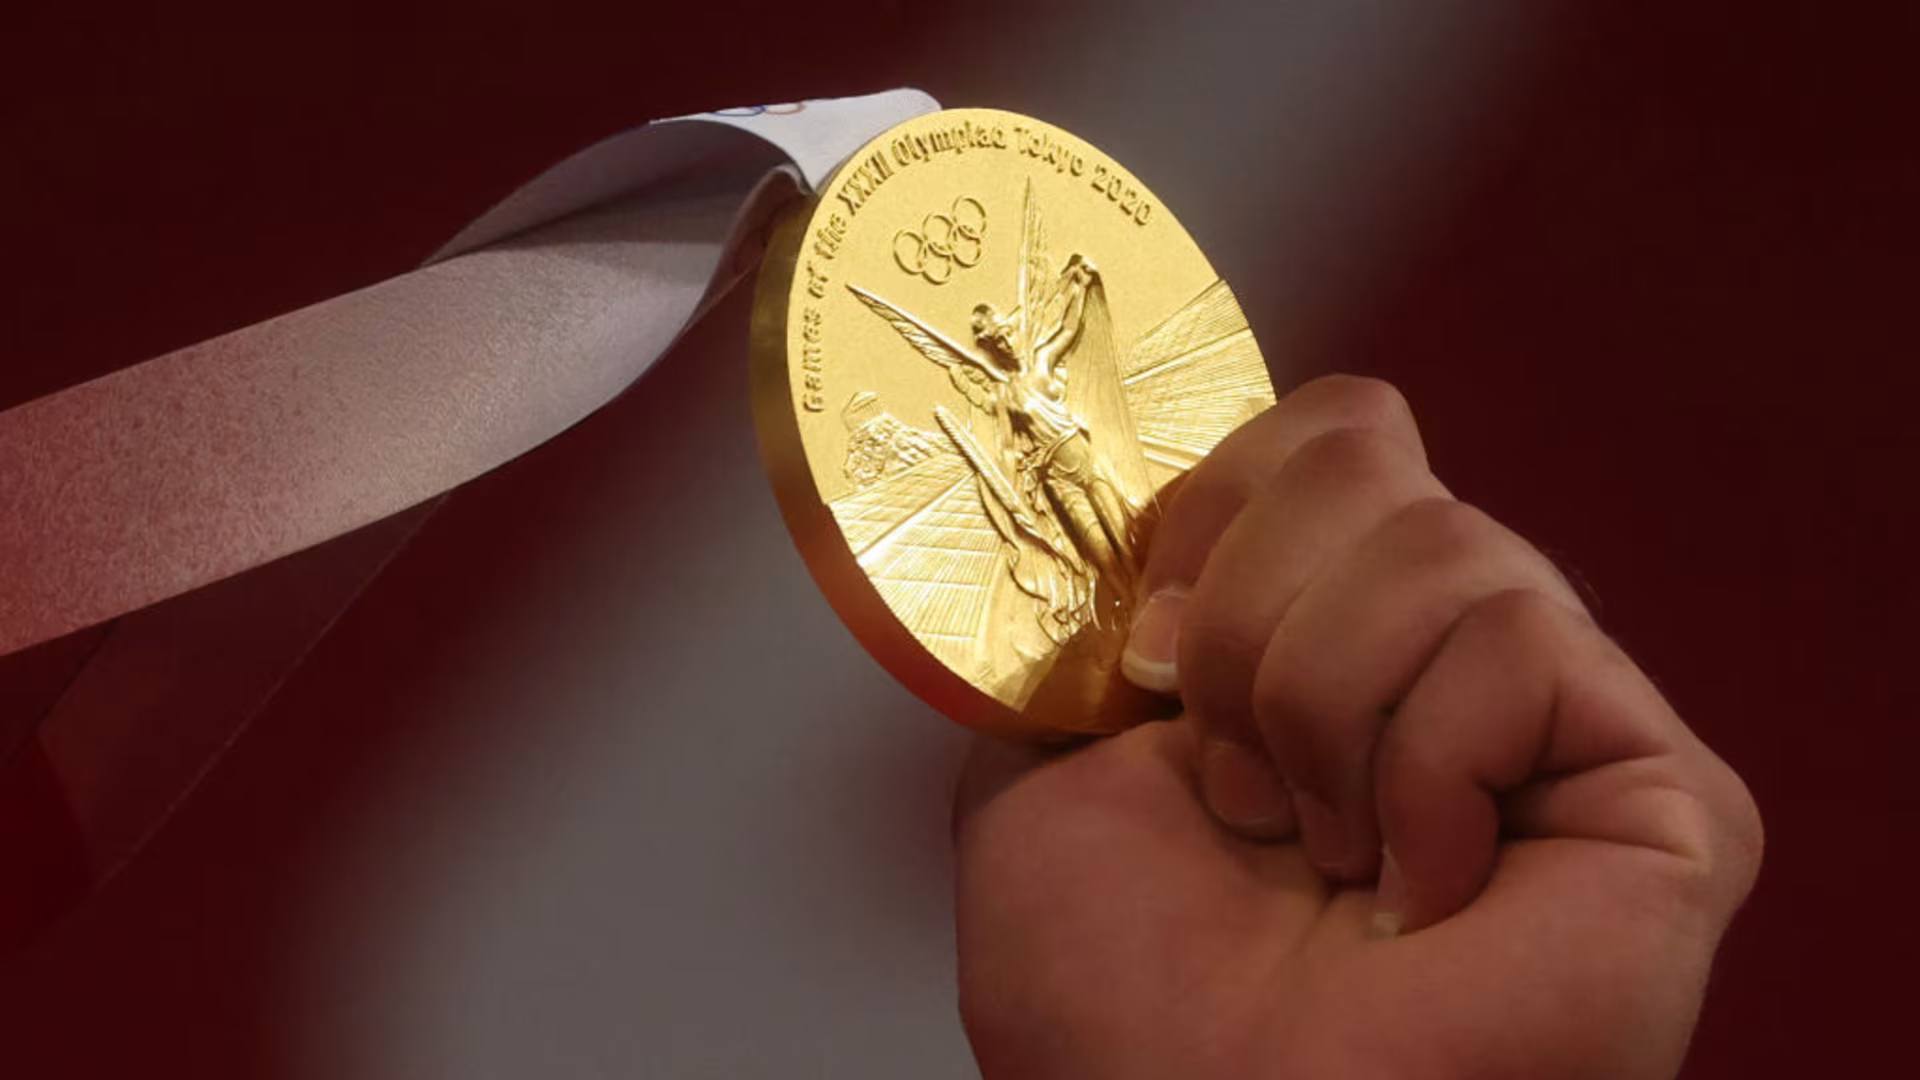
\includegraphics[width=0.7\linewidth]{fig/background}
	\caption{}
	\label{fig:background}
\end{figure}











\subsection{Restatement and Analysis of the Problem}










\subsection{Ovirview of Our Work}

\begin{itemize}
	\item {\bf 111}. ...
	\item {\bf 222}. ...
	
	\begin{itemize}
		\item[1)] ... 
		\item[2)] ...
		\item[3)] ...
		\item[4)] ...
	\end{itemize}
	
\end{itemize}








%%%%%%%%%%%%%%%%%%%%%%%%%%%%%%%%%%%%%%%%
%%%%%%%%%%%%%%%%% 模型假设 %%%%%%%%%%%%%%%%%
%%%%%%%%%%%%%%%%%%%%%%%%%%%%%%%%%%%%%%%%
\section{Assumptions and Justification}

To simplify the problem and make it convenient for us to simulate real-life 
conditions, we make the following basic assumptions, each of which is properly 
justified.

\begin{itemize}
	\item {\bf 111}. ...
	\item {\bf 222}. ...	
\end{itemize}










%%%%%%%%%%%%%%%%%%%%%%%%%%%%%%%%%%%%%%%%
%%%%%%%%%%%%%%%%% 符号说明 %%%%%%%%%%%%%%%%%
%%%%%%%%%%%%%%%%%%%%%%%%%%%%%%%%%%%%%%%%
\section{List of Notations}
\begin{center}
	\begin{tabular}{clc}
		\toprule
		{\bf Symbols} & {\bf Description} & \quad {\bf Unit} \\
		\midrule 
		$h$ & Convection heat transfer coefficient & \quad W/(m$^2 \cdot$ K) \\[0.2cm]
		$A$ & Aera & \quad m$^2$ \\[0.2cm]
		$a,\,b,\,c$ & The size of a bathtub  & \quad m$^3$ \\
		\bottomrule
	\end{tabular}
\end{center}

\noindent where we define the main parameters while specific value of those 
parameters will be given later.


%%%%%%%%%%%%%%%%%%%%%%%%%%%%%%%%%%%%%%%%
%%%%%%%%%%%%%%%%% 数据预处理 %%%%%%%%%%%%%%%%%
%%%%%%%%%%%%%%%%%%%%%%%%%%%%%%%%%%%%%%%%
\section{Data Pre-processing}
\subsection{Outlier Handling}
No obvious outliers were observed in the data. However, Skating and Ice Hockey have been included in the Winter Olympics since 1920, so these two events are not within the scope of consideration.



\subsection{Missing Value Handling}



\subsection{Tag Encoding of String Type Data}


%%%%%%%%%%%%%%%%%%%%%%%%%%%%%%%%%%%%%%%%
%%%%%%%%%%%%%%%%% Task 1 %%%%%%%%%%%%%%%%%
%%%%%%%%%%%%%%%%%%%%%%%%%%%%%%%%%%%%%%%%
\section{Task 1: xxx}

\section{Task 2: xxx}

\section{Task 3: xxx}

\section{Task 4: xxx}

\section{Sensitivity Analysis}

\section{Strength and Weakness}
\subsection{Strength}
\subsection{Weakness}

\section{Further Discussion}




%% 表格
%\begin{table}
%\centering
%\caption{}
%\label{fig:missing_value}
%\begin{tabular}{cc}
%\toprule
%{\bf Discipline} & {\bf Code} \\
%\midrule
%Jeu de Paume & JDP
%\end{tabular}
%\end{table}

























% 因为不输出此部分到目录 \addcontentsline{}{}{}是添加此标题到目录 
\newpage
% 美赛中不能出现中文,中文参考文献可自己翻译成英文
\section*{References}\addcontentsline{toc}{section}{References}
\fancyhf{}
\fancyhead[R]{ }
\fancyhead[L]{ }
\bibliography{reference}
\Large
\bibliographystyle{IEEEtran}

\newpage
\section*{Appendices\addcontentsline{toc}{section}{Appendices for Code and Data}}


\end{document}